\begin{center}
    % \vspace{-0.2in}
\begin{tabular}{cccc}
  \toprule
  Trajectory generation policy & UCB & TS & policy gradient \\
  \midrule
  no offline dataset                           & 1691.827 & 163.483 & 858.794 \\
  offline, no enlarge                          & 1303.405 &  43.550 &  82.254 \\
  offline+copy                                 & 1156.635 &  26.596 &  54.048 \\
  offline+diffuse pair                         & 1028.613 &   7.296 &  42.993 \\
  offline+diffusion sequence                   &  923.779 &   0.071 &   3.522 \\
  offline+diffusion sequence (Transformer)     &  743.441 &   0.008 &   0.002 \\
  \bottomrule
\end{tabular}
    \captionof{table}{Performance(average accumulated regret) of various algorithms on Bernoulli-reward bandits under different offline-dataset enlargement (trajectory-generation) policies.}
    % \vspace{-0.45in}
\end{center}


\begin{tikzfigure}[Performance of each algorithm(UCB, policy gradient) across arm counts(20, 25, 30) with non-Bernoulli rewards, evaluated under three pre-training settings: none, offline (500 trajectories generated by diffusion sequence (Transformer).]
    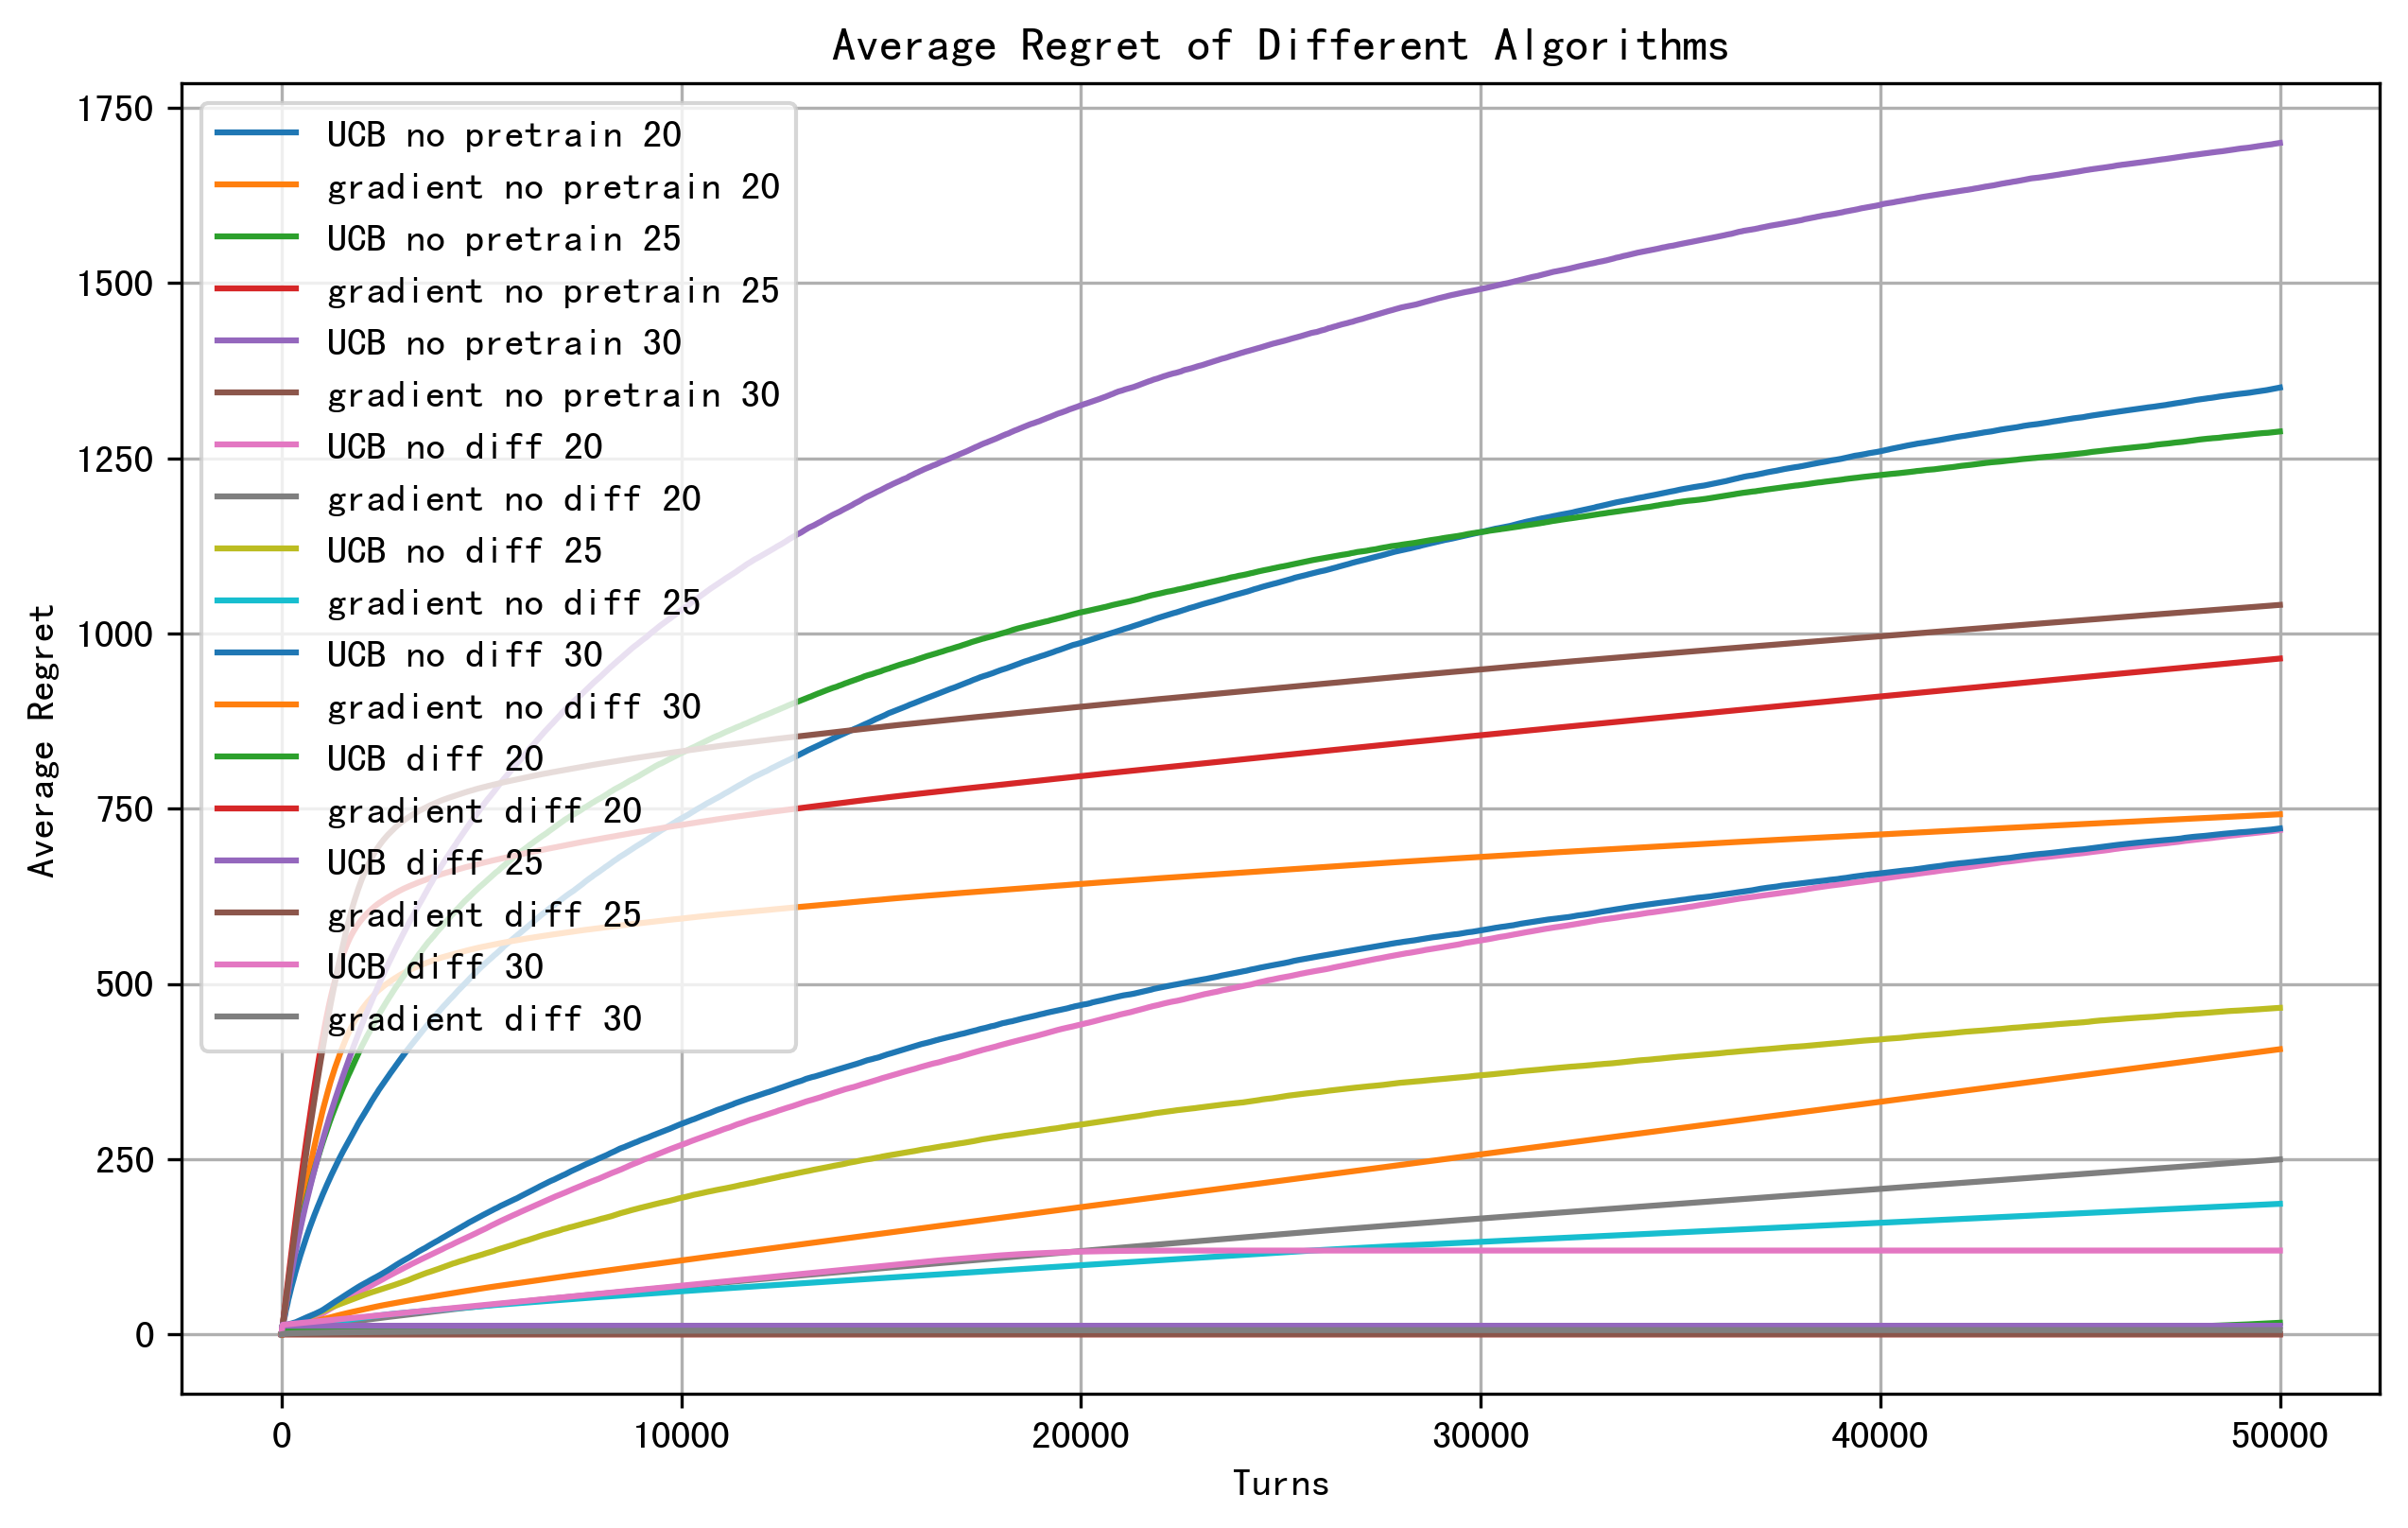
\includegraphics[width=\linewidth]{./Img/stochastic_non_bern.png}
    % \vspace{-1in}
\end{tikzfigure}